%% ---------------------------------------------------------------------------
%% intro.tex
%%
%% Introduction
%%
%% $Id: intro.tex 1477 2010-07-28 21:34:43Z palvarado $
%% ---------------------------------------------------------------------------

\chapter{Introduction}
\label{chp:intro}

Computers were invented to accelerate manual processes. In the beginning, computers
offered speeds far superior than what a human could manage on specific activities, but their use
was limited to relatively low data processing. 

In the current era of increasingly advanced semiconductor technologies, a need for using computers 
with applications for high-level data processing has risen along with higher amounts of data to process.
This has generated a race for maintaining high performance while keeping equal or even reduced 
energy, time and storage consumption. The main solution, for some years, has been to increase the 
computing power of the computers via mechanisms such as, for example, increasing the number of transistors
per area. This solution, however, has brought with it a lot of considerations and problems, specially 
regarding energy consumption.

A new approach has surfaced as one of the solutions to the energy consumption problem is, approximate computing.
This computing paradigm was born on the assumption that there are cases on which an exact result, with high precision,
is not needed. A lot of data comes from inexact sources (sensors, readings) or do not require a precise processing
algorithm (machine learning, user recommendation programs, statistics). This type of applications is
known as error-tolerant. Approximate computing looks to use these types of data to create algorithms,
languages, compilers, circuits and computer architectures that have the common objective of lowering
the energy consumption and increasing the performance at the cost of having an approximate result.

Machine learning is a current area of research that can take advantage of the benefits of approximate
computing. Its main property is
decision making based on processing big amounts of data. This data can be written, visual (images, video) or 
audio information, as well as taking the feedback into account to improve the learning process.
Approximate computing can take advantage of this fact and use it to reduce the computational effort
required and, in this manner, improve significantly the investigation area of machine learning.

This work looks to explore methods and techniques for approximate hardware definition on FPGA, such that
it could be used on machine learning applications, specifically by generating approximate hardware
kernels for CNNs through the use of OpenCL. The current project will deliver useful tools for any 
other developer that requires to accelerate their machine learning algorithms through the use of FPGAs.

\section{Project background}

\subsection{Organization}

The project is developed in the KIT, a university focused on the development of technology and science.
KIT was created on 2009 after the convergence of the University of Karlsruhe, funded on 1825, and the 
Investigation Center of Karlsruhe. It is located in Karlsruhe, in the Baden-Württemberg state, to the
southwest of Germany. Figure \ref{fig:mapakit} shows a map with the location of Baden-Württemberg inside the european
country and the location of Karlsruhe inside the aforementioned state.

\begin{figure}[H]
    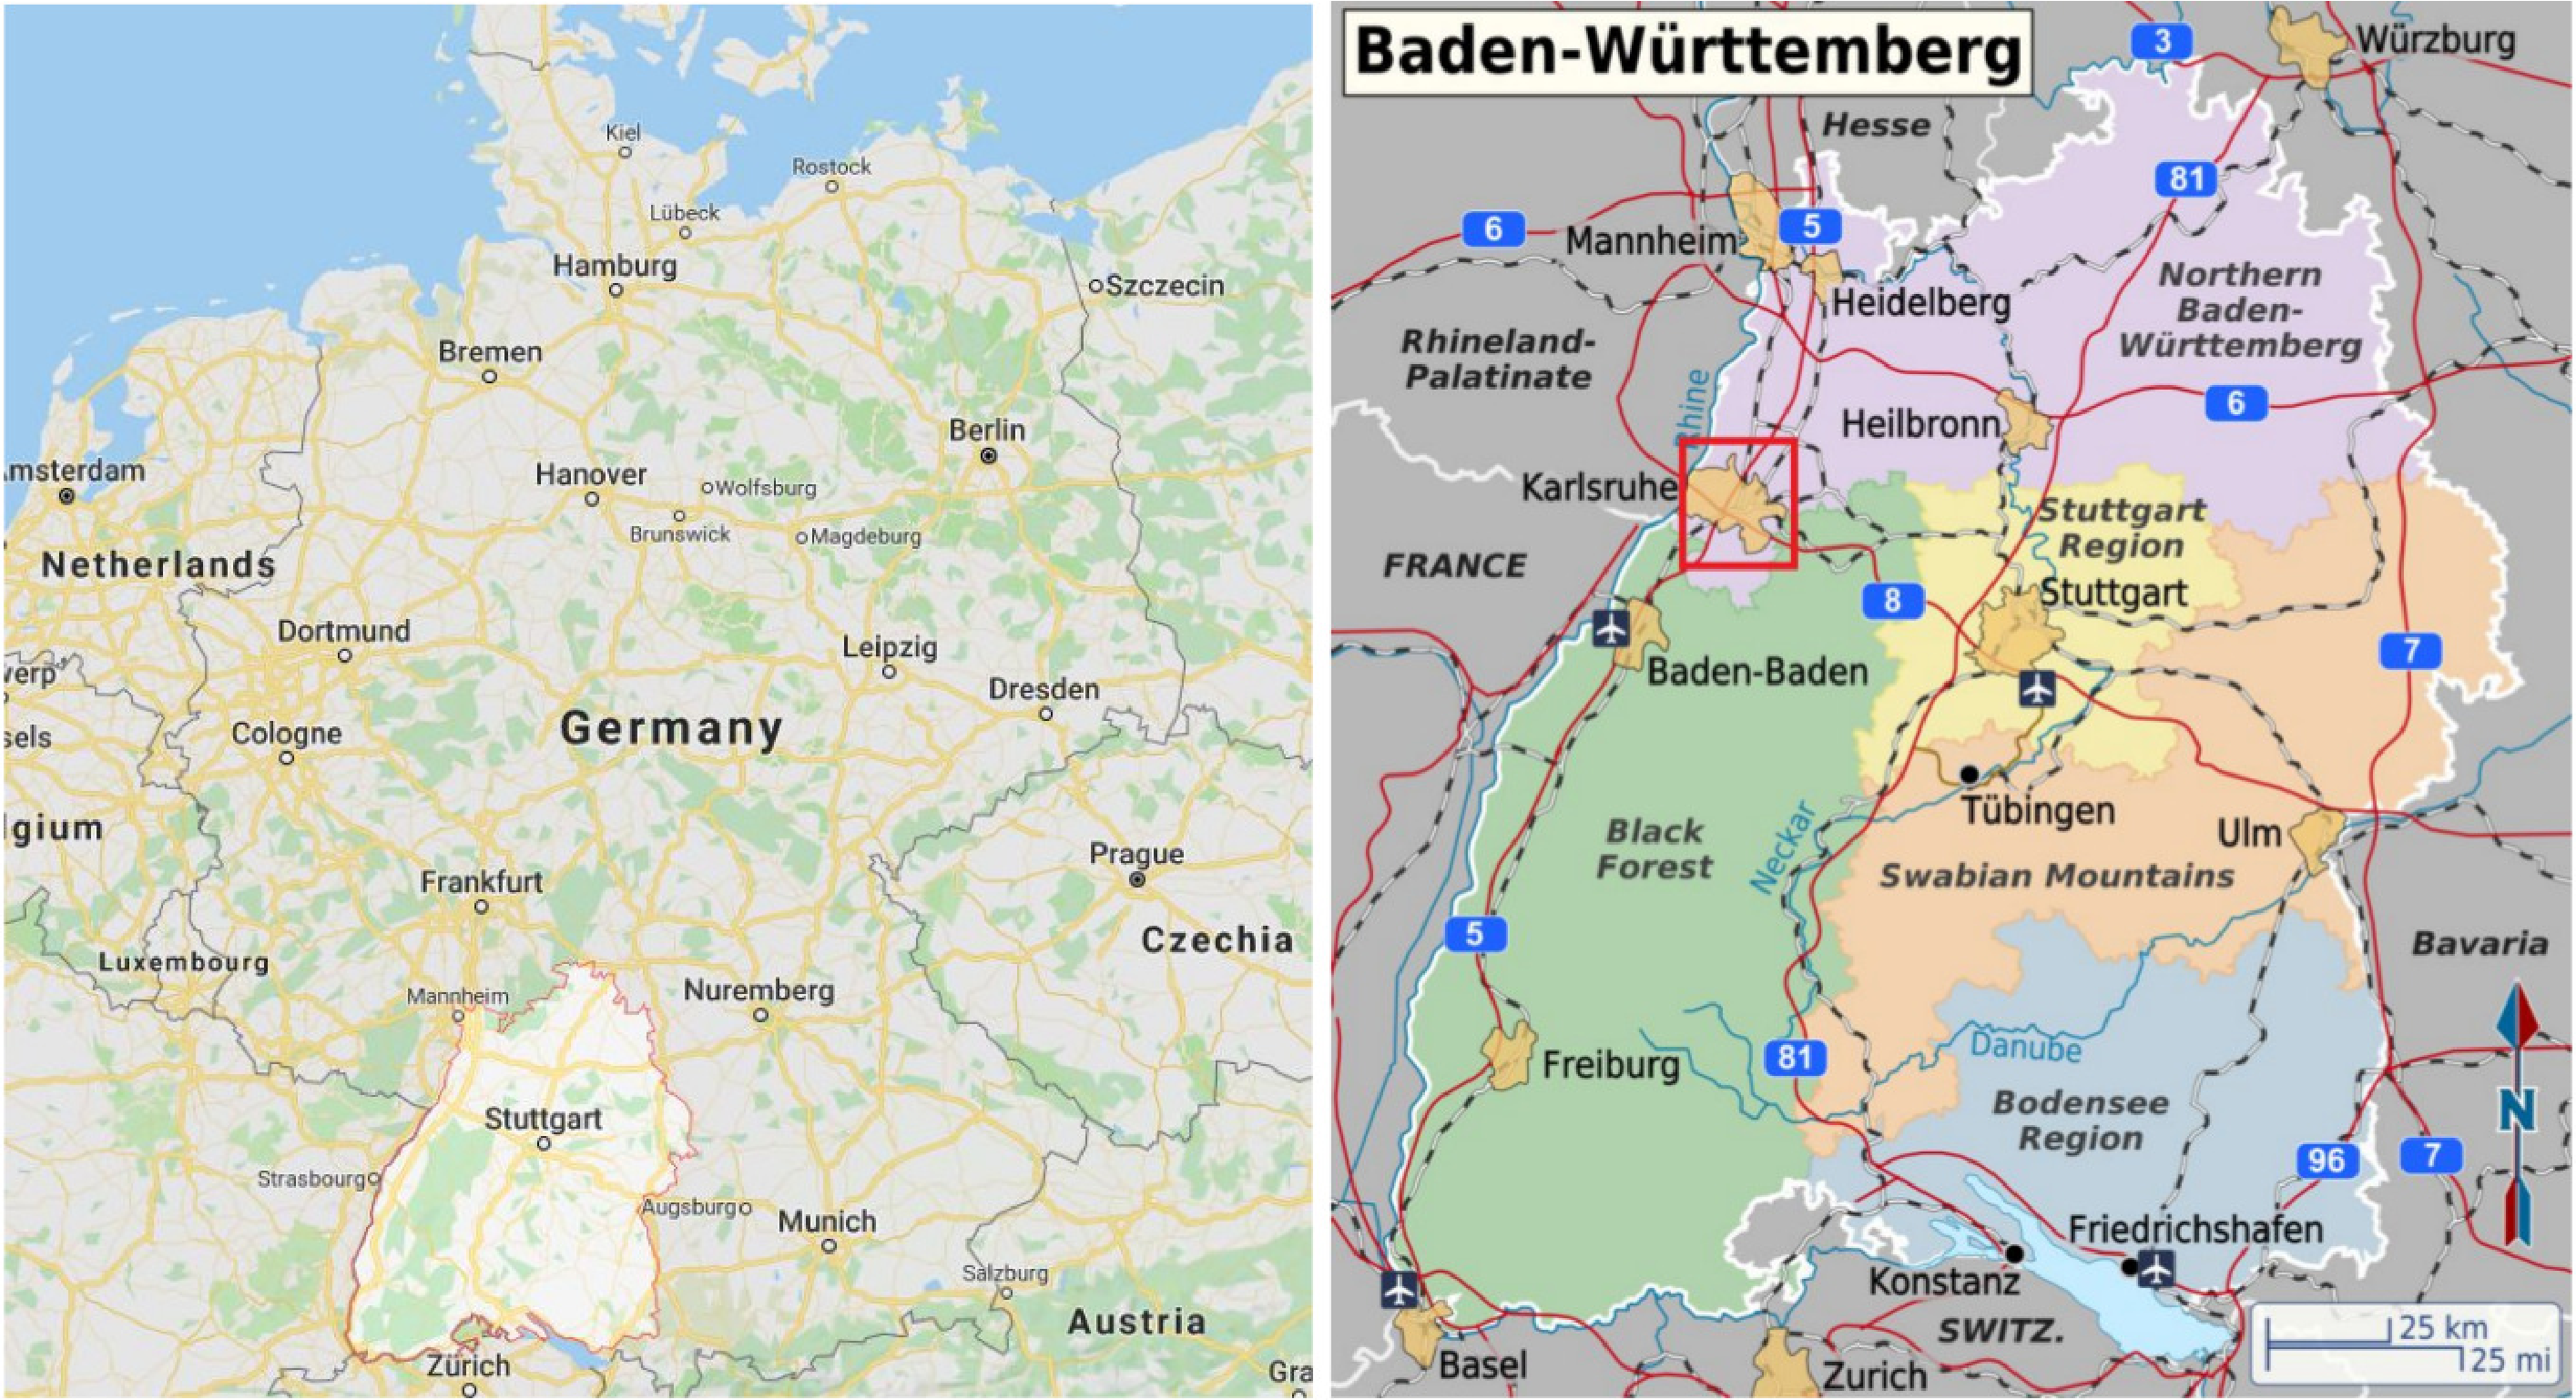
\includegraphics[width=\linewidth]{fig/mapakit.eps}
    \caption{Map of Germany with Baden-Wüttemberg marked (left) \cite{badenmap} and location of Karlsruhe within the state (right) \cite{karlsmap}}
    \label{fig:mapakit}
\end{figure}

Nowadays, KIT is one of the most prestigious technical universities in Germany, specializing on engineering
and science. Figure \ref{fig:kitlogo} shows the current logo of the university. KIT is conformed by a scientific organization
separated by divisions:

\begin{compactitem}
    \item Division I: Biology, Chemistry and Process Engineering.
    \item Division II: Informatics, Economy and Society.
    \item Division III: Mechanical and Electrical Engineering.
    \item Division IV: Natural and Built Environment.
    \item Division V: Physics and Mathematics.
\end{compactitem}

\begin{figure}
    
\includegraphics[width=\linewidth]{fig/kitlogo.eps}
    \caption{Logo of the Karlsruher Institut für Technologie \cite{kitlogo}}
    \label{fig:kitlogo}
\end{figure}

These divisions are constituted by departments destined to investigational work, innovation and teaching.
Each department has institutes responsible for university education. Aside from the institutes, there are
KIT centers, on which topics related to investigation and innovation go beyond the divisions, supporting
an interdisciplinary cooperation \cite{kitorg}. 


The Department of Informatics is one of the first to be established on Germany. This department is formed
by different institutes focused on teaching and investigation of topics associated with informatics. As
part of the Department of Information the CES comes as a center of investigation on aspects related
with the design of embedded systems, from the reliability of electrical circuits to the management of
electrical power on systems with multiple and many cores.

\subsection{Knowledge area}

The project is developed within the technical area of approximate computing, which is part of the areas
of interest of computer engineering. Approximate computing looks to relax the numerical equivalence 
between the specification and implementation of such applications promising significant 
energy-efficiency improvements and it has gained significant traction over the past few years \cite{surveyqu}. Within
approximate computing, the project focuses on the utilization of \intelOCL  to develop approximate hardware
kernels and their application on CNNs. The goal is to highlight the effect of these kernels on the improvement in 
performance and reduction on resource usage in comparison to exact kernels.

This kernels must be designed using high-level synthesis tools. OpenCL is a tool that allows to define 
procedures on heterogeneous platforms through the 
use of a high-level programming language. The knowledge on hardware changes via the use of a software 
description is necessary to develop the project.

\subsection{Similar works}

In the area of neural network implementation on FPGA using OpenCL, notable previous works are:
\begin{itemize}
    \item Suda et al. introduce a complete OpenCL-based accelerator design for CNNs based on
    matrix multiplication. They also explain algorithms to apply convolution by rearranging
    the components of the input image. This work is an exact CNN that could be used as a base
    for the current project. \cite{suda}
    \item Wang et al. propose a CNN implementation on FPGA specifically taking advantage of 
    the ability to allow communication between layers through data channels \cite{pipecnn}.
    \item Zhang and Li present a model to analyze the resource usage on an FPGA, as well as
    implementing their own accelerator based on OpenCL \cite{zhangcnn}.
\end{itemize}

Regarding the use of approximate computing for CNNs, we can find the following related works:
\begin{itemize}
    \item Moons et al. show that using approximations on popular CNNs can increase the energy
    efficiency of the accelerators and show some of the techniques that can be applied to other
    CNNs \cite{moons}.
    \item Kamel et al. compile a lot of techniques that can be used on CNNs and some other 
    information regarding the application of CNNs on FPGAs \cite{kamel}.
\end{itemize}

Also, there is the work done by D. Spies [reference missing as the thesis has not been published yet]
on which some CNN frameworks were implemented for low-power FPGAs, reducing the need for high-end
FPGAs and allowing for further research on the area.

\section{Problem statement}

\subsection{Problem context}

In the last years, discussions on the physical (and economical) limits of the very-large-scale integration 
of transistors have surfaced \cite{aftermoore}\cite{moorelawlimit}, where statements like Moore's Law exert pressure the big chip manufaturers.
Gordon Moore himself has assured that this trend cannot be maintained for a long time \cite{mooredead}. This leads to the
search of new paradigms or techniques that allow to sustain the high requirements on performance and 
energy consumption of applications in the technological world, where a need to process even higher amounts
of data is increasing. Some solutions to this increasing demand have appeared, such as multicore computers,
multithreading architectures, large scale computers, GPU processing and more.

Despite these solutions, there exist other problems that cannot be solved just by improving on the architecture
of the processor. Some of these problems are:

\begin{compactitem}
    \item The memory wall: Wulf and McKee \cite{memorywall} describe an imminent problem on which the superior speed increase
    of the processors is a lot higher that the improvement on memory technologies. This requires solutions that
    try to reduce the amount of memory accesses.
    \item The utilization wall: Taylor et al. \cite{utilizationwall} noticed a phenomenon that appears due to the increase on the amount
    of transistors per unit of area in a chip. The problem is related to an exponential reduction of the usable
    percentage of the chip depending on the scale of integration of the transistors.
    \item Problems with thermal dissipation: with the increase of frequency of the microprocessors, the level of 
    heat dissipation has increased, forcing a reduction on the operational voltage. Some solutions have been proposed
    to this problem, like the utilization of multicore processors with cores that deactivate themselves to reduce
    the workload \cite{whitepaper}.
\end{compactitem}

Approximate computing tries to solve this type of problems with the help of the recent increase of error-resilient
applications (e.g. \cite{errortolerant}). This paradigm tries to eliminate, or reduce, the need for precision
during processing with the goal of obtaining gains in energy efficiency and processing speed.

Furthermore, one area of interest within the error-resilient application world is machine learning.
The goal of this area is to allow a computational system to execute tasks without the need for a prior
specific programming and, in some cases, using previous results as feedback to improve the execution.
Algorithms used in machine learning look to build mathematical models based on "training" data to perform
tasks without explicit programming \cite{patternrecogbook}. Due to their nature, machine learning applications do not present
an exact response immediately, or even never, instead they require multiple feedback cycles to achieve
the expected response. This means that approximate computing is a potential paradigm to work with this
type of applications \cite{approximatecomp}.

\subsection{Justification of the problem}

Approximate computing is an area that is still in the upswing. There are diverse investigations and designs
that look to take advantage of the existence of error-tolerant applications. However, it is necessary to
continue advancing the paradigm and develop new techniques in order to observe its contributions in daily
life. The importance of this paradigm resides on the fact that it does not depend on the current state
of the technology to bring forth energetic and performance improvements.

The use of FPGA in the area of approximate computing is still under explored. At the same time, machine
learning applications are of great interest to a lot of fields. An improvement on current machine learning
implementations through the combination of both areas would generate new opportunities and solutions
with low energetic consumption and high adaptability levels. Following this thought, the project is
important due to the following:

\begin{compactitem}
    \item It allows to advance the investigation on the area of approximate hardware definition
    using popular tools such as OpenCL, which could be used as the basis for future investigations
    with FPGA based applications.
    \item The use of a popular and easy to use tool could speed up the generation of results in a
    less explored area, such as FPGA implemented neural networks.
    \item The project generates new tools easily adaptable to machine learning applications based
    on neural networks. These tools can be individual kernels or sets of customizable kernels. 
    \item New investigations on error tolerant applications and approximate computing can easily 
    make use of the findings of this project.
\end{compactitem}


\subsection{Problem definition}

Machine learning applications are based on different methods used to obtain results.
One of the most used techniques are called neural networks, with the objective of imitating the work
done by the human brain to obtain similar results. Furthermore, there is a branch of neural networks
called deep learning. It consists in the increase of the amount of processing layer in order to obtain
a bigger amount of details from an input of data \cite{deeplearningoverview}. Layers are represented by nodes (neurons)
that process data from the input. This processing requires a high level of computation, but its
results are mostly approximations. CNNs are part of the deep learning neural network implementations, with most
of its usage focused on analyzing input images.

Now, FPGAs are devices that have been recently the object of investigations with the objective of accelerating
the current processing being done. The interest in using FPGAs for high amounts of computation comes from
the limitation of general use CPUs, which do not offer enough processing power (multiple operations with 
high level of complexity at the same time); and GPUs that, even with the capability of processing high
amounts of data at the same time, are not specialized enough or even customizable to perform specific tasks.
The use of a device that can be programmed at the hardware level for specific tasks (in this case, neural networks)
offers possibilities on processing speed and energy efficiency that surpass GPUs \cite{surveyfpgann}.

The current project emerges with the objective of contributing to the ongoing investigation efforts
in the area of FPGAs for machine learning applications through approximate hardware definition.
Each neuron in a neural network is represented as a "hardware kernel" that gets defined the 
calculations and processes that it needs to do on the input data to analyze it.
Through the use of software tools like OpenCL, it is possible to define kernels that perform
machine learning tasks. Combining all these areas and tools, an improvement on performance and
energy consumption must be possible, allowing machine learning applications to keep up
with the global demand for higher amounts of data processing.


\section{Objectives}

The project tries to find a solution to the ever increasing energy consumption problem
of current world technologies. This is accomplished by using low energy platforms such as
FPGAs applied to CNNs with the use of high-level definition tools like OpenCL.

\subsection{Main objective}

Design an approximate hardware implementation of CNNs through the 
use of \intelOCL.

\subsection{Specific objectives}

\begin{compactitem}
    \item Describe the viable changes on the OpenCL tool for approximate hardware generation on FPGA.
    \item Create approximate and reusable hardware kernels for CNNs using OpenCL.
    \item Determine the error-tolerance level of CNNs when using approximate kernels instead of exact kernels.
    \item Ascertain the reduction of computational resources when using approximate kernels compared to the use of traditional exact kernels.
\end{compactitem}

\section{Scope, deliverables and limitations}

\subsection{Scope}

The project's end goal is designing, developing and implementing approximate hardware kernels on FPGA.
These kernels represent each of the layers of a CNN and will allow for an image processing algorithm to be
performed on them. The end result must be more energy efficient and provide better performance over existing
implementations of CNNs.

The project is subdivided in the following stages:

\subsubsection{Theoretical investigation}

A first step is to investigate on the following topics:

\begin{itemize}
    \item Convolutional neural networks.
    \item OpenCL and hardware definition.
    \item Approximate computing on neural networks.
    \item CNN implementation on FPGAs.
\end{itemize}

This will provide the necessary information to use OpenCL to implement CNNs on FPGA.
Futhermore, this information can also be used to generate mathematical models to measure the error
and precision of the generated CNNs, be them exact of approximate, as well as the comparison between
both implementations.

\subsubsection{Exact CNN implementation on FPGA}

An exact CNN implementation must be developed in order to have a baseline
to develop the approximate kernels. This exact CNN implementation is also used to
compare results in order to evidence the performance and energy efficiency improvements.
Finally, the approximate CNN implementation must be a modification of the exact model.

\subsubsection{Approximate CNN implementation on FPGA}

This implementation must be completely based of the exact CNN implementation and will 
reflect the OpenCL changes that allow for a different hardware definition, one that is 
approximate and adds errors in the processing of the input data. Also, the approximate
implementation must have a set maximum error, which should be measurable and used
in the mathematical models.

\subsubsection{Comparison against base implementation}

Using the results of both the exact and approximate implementation, an analysis of
the effects of approximate modifications against the exact implementation must be performed.
This analysis should reflect which approximate changes are better in terms of performance gain,
reduction of resource usage and accuracy loss.

\subsection{Deliverables}

\begin{enumerate}
    \item Theoretical investigation
        \begin{enumerate}
            \item Compilation report of the use of neural networks on FPGA: this report will contain
            relevant information to be used in the rest of the project and will guide the decision
            making when designing neural networks on FPGA. 
            \item Progress report with the viable modifications: report with the modification possibilities
            with OpenCL and that affect the hardware definition on FPGA.
        \end{enumerate}
    \item Design stage
        \begin{enumerate}
            \item Documentation on how to approximate neural networks: contains the necessary information
            on the principles of approximate computing that are applicable on neural networks, specifically
            for CNNs. It should contain mathematical models that can be compared against the results
            of the project.
            \item Design of the error calculation model: contains the mathematical formulations that allow
            to create a precise calculation of the results that will be obtained so they can be compared
            with the gain in performance.
        \end{enumerate}
    \item Code development
        \begin{enumerate}
            \item Source code: source code of the OpenCL application and any other code necessary to
            compile, execute and test the kernels.
            \item Exact kernels: source code of the exact kernels used as a base line for the approximate kernels.
            \item Approximate kernels: source code of the approximate hardware kernels that will be used
            on the testing phase.
        \end{enumerate}
    \item Testing stage
        \begin{enumerate}
            \item Results of the exact tests: measurements of performance, precision and resource usage while
            testing the exact kernels.
            \item Results of the approximate tests: measurements of performance, precision and resource usage while
            testing the approximate kernels.
            \item Results documentation: comparison of the results between exact and approximate tests.
        \end{enumerate}
    \item Project administration
        \begin{enumerate}
            \item Design document: contains the design of every tool developed during the project.
            \item Meeting minutes: contains all information obtained in the progress and validation
            meetings.
            \item Final report: final report of the project with all relevant information that was
            generated during its course.
        \end{enumerate}
    
\end{enumerate}

\subsection{Limitations}

LIM-01: the student must mobilize to Germany in order to reduce conflicts with the project supervisor.
Because of the lack of a visa, the time in the european country is limited to 3 months. 
 
LIM-02:​ the student's budget is only 1000 euros during the stay in Germany. This money will only cover feeding, staying and commuting costs,
limiting the possibility of buying new tools to develop the project. The student must use any tools that the supervisor or the university
can give him.

LIM-03: the student must comply with the regulations and limitations of the KIT regarding international
students.

LIM-04: no face to face meetings are possible with the advisor teacher due to the geographical location of 
the student during the project. Due to timezone differences, the available times for meetings is limited
to 8 hours or less per day and the meetings depend on having good internet service and working
audio equipment.

LIM-05: as the student does not have access to a computer with a middle to high end GPU, the base software
implementation of the CNN is limited to CPU only.

LIM-06: some of the changes to be done on the CNN are changes to the original definition of the network.
These changes may require a new training phase for the network which represents weeks on training.
Any approximation proposed must work with the existing training weights for the selected CNN.

% \subsection{Risks}

% RIE-01: ​ Recibir un rechazo de la solicitud de la visa. El proceso de solicitud de visa ya fue iniciado, pero
% existen diversos factores que pueden hacer que la visa sea rechazada y que están fuera del control del
% estudiante.
% - Probabilidad: media. Existe un antecedente de la extensión de solicitud de visa por parte de otro
% estudiante que realizó el mismo viaje hacia Alemania.
% - Impacto: medio. El no tener visa significa que el tiempo de estadía en Alemania se reduce a 3
% meses. El tiempo no se reduce demasiado, pero eso añade una presión extra al estudiante y
% reduce el tiempo efectivo de desarrollo del proyecto.
% - Acciones mitigadoras: se va a iniciar el proyecto con la sección de investigación un tiempo antes
% del viaje hacia Alemania para reducir el impacto de una reducción del tiempo de estadía.

% RIE-02: No conseguir un lugar de residencia para la fecha de llegada a Alemania. Los procesos de
% obtención de residencia en Alemania contienen diversos pasos, entre ellos una entrevista personal que
% supone una mayor dificultad para obtener un lugar de estadía.
% - Probabilidad: baja. A pesar de que cada lugar tiene diferentes procesos, existen muchas
% opciones de estadía y el precio de alquiler no supone un riesgo para el proyecto. Además,
% existen opciones para alojarse mientras se busca una estadía permanente.
% - Impacto: bajo. De no encontrar un hospedaje para la fecha de llegada, el estudiante deberá
% disponer de tiempo de desarrollo del proyecto para conseguir el hospedaje.
% - Acciones mitigadoras: el estudiante debe agotar todas las opciones existentes de hospedaje
% meses antes del viaje a Alemania para aumentar las posibilidades de conseguir alojamiento.
            
% RIE-03: El estudiante deberá obtener un vuelo que se adapte a las necesidades de fecha de inicio de las
% tareas en Alemania y a las limitaciones de tiempo impuestas por la visa (o falta de ella). Debido a que los
% vuelos suponen un complejo sistema de escalas y destinos, existe un riesgo de obtener un vuelo que
% llegue a Alemania en una fecha posterior a la prevista.
% - Probabilidad: baja. Existen múltiples opciones para conseguir vuelos que se adapten a las
% diferentes necesidades de las personas.
% - Impacto: baja. El proyecto se podría retrasar varios días.
% - Acciones mitigadoras: se debe obtener un vuelo que satisfaga las necesidades del estudiante
% con anticipación y estar atento a nuevas opciones.

% RIE-04: La universidad KIT permite a todo estudiante admitido ser registrado en ella. Esto ofrece
% beneficios específicos para estudiantes matriculados en universidades alemanas, como descuentos en
% transporte público. El riesgo está en que el registro no pueda ser completado.
% - Probabilidad: baja. El estudiante ya fue admitido en la universidad y el cumplir con todos los
% requisitos reduce la posibilidad de que el registro sea rechazado.
% - Impacto: baja. El no ser registrado podría provocar un aumento en los gastos financieros del
% estudiante,. Sin embargo, esto no supone mayor inconveniente.-
% Acciones mitigadoras: el estudiante ha ahorrado dinero extra en caso de necesitar realizar
% gastos mayores de los esperados.

% RIE-05: El proyecto depende de que la herramienta de software permita modificaciones adecuadas para
% la definición de hardware aproximado en FPGA. Un riesgo del proyecto es que la herramienta no
% permita realizar definición de hardware no exacto.
% - Probabilidad: media. La herramienta a utilizar es Intel® FPGA SDK for OpenCLTM. Este es un
% framework de código-cerrado.
% - Impacto: medio. De no ser capaz de utilizar OpenCL para desarrollar el proyecto, se deberá
% acudir a otras opciones, esto retrasaría el proyecto.
% - Acciones mitigadoras: el estudiante deberá buscar otras opciones antes de iniciar el proyecto
% para evitar un bloqueo en el proyecto.

% RIE-06: De ser capaz de realizar modificaciones en la definición de hardware obtenida por parte de la
% herramienta, existe el riesgo de que estas modificaciones no sean suficientes para obtener hardware
% aproximado para kernels de redes neuronales.
% - Probabilidad: media. Esta es una de las mayores incertidumbres del proyecto y parte de los
% resultados de la investigación teórica.
% - Impacto: alto. El no ser capaz de realizar modificaciones para obtener hardware aproximado
% significa un replanteamiento por completo del proyecto.
% - Acciones mitigadoras: la primera tarea que debe realizar el estudiante es investigar las
% diferentes modificaciones que se deben realizar para reducir la incertidumbre del proyecto.

% RIE-07: Con la suposición de que es posible aproximar el hardware generado por la herramienta de
% software, aparece el riesgo de que la aproximación realizada en redes neuronales no permita tener un
% error suficientemente aceptable en los resultados prácticos de los algoritmos de aprendizaje.
% - Probabilidad: baja. Existen diversos estudios que tratan el tema de aproximación de redes
% neuronales.
% - Impacto: medio. Aunque no se obtenga un resultado positivo en algoritmos de aprendizaje, el
% proyecto puede tener resultados que permitan potenciar otras investigaciones.
% - Acciones mitigadoras: el estudiante deberá mantenerse informado con respecto a las
% posibilidades de mejora en redes neuronales así como los niveles de error que pueden ser
% considerados como aceptables.

%%% Local Variables: 
%%% mode: latex
%%% TeX-master: "main"
%%% End: 
